\chapter{Attachments}
\begin{figure}
\caption{All possible values representing an operator in an instance of \texttt{OperatorNode}}
\label{FIG_operators}
Logical: \texttt{AND}, \texttt{OR}.

Comparison: \texttt{GEN\_EQUALS}, \texttt{GEN\_NOT\_EQUALS}, \texttt{GEN\_LESS\_THAN}, \texttt{GEN\_LESS\_THAN\_EQUALS}, \texttt{GEN\_GREATER\_THAN}, \texttt{GEN\_GREATER\_THAN\_EQUALS}, \texttt{VAL\_EQUALS}, \texttt{VAL\_NOT\_EQUALS}, \texttt{VAL\_LESS\_THAN}, \texttt{VAL\_LESS\_THAN\_EQUALS}, \texttt{VAL\_GREATER\_THAN}, \texttt{VAL\_GREATER\_THAN\_EQUALS}, \texttt{NOD\_IS}, \texttt{NOD\_PRECEDES}, \texttt{NOD\_FOLLOWS}.

Range: \texttt{TO}.

Additive: \texttt{PLUS}, \texttt{MINUS}.

Multiplicative: \texttt{MUL}, \texttt{DIV}, \texttt{IDIV}, \texttt{MOD}.

Set: \texttt{UNION}, \texttt{INTERSECTION}, \texttt{DIFFERENCE}.

Type test: \texttt{INSTANCE\_OF}, \texttt{CASTABLE\_AS}.

Type conversion: \texttt{TREAT\_AS}, \texttt{CAST\_AS}.

Unary: \texttt{UNARY\_PLUS}, \texttt{UNARY\_MINUS}.
\end{figure}

\begin{figure}
\caption{XSD built-in atomic types.}
\label{FIG_xsd_built_in_atomic_types}
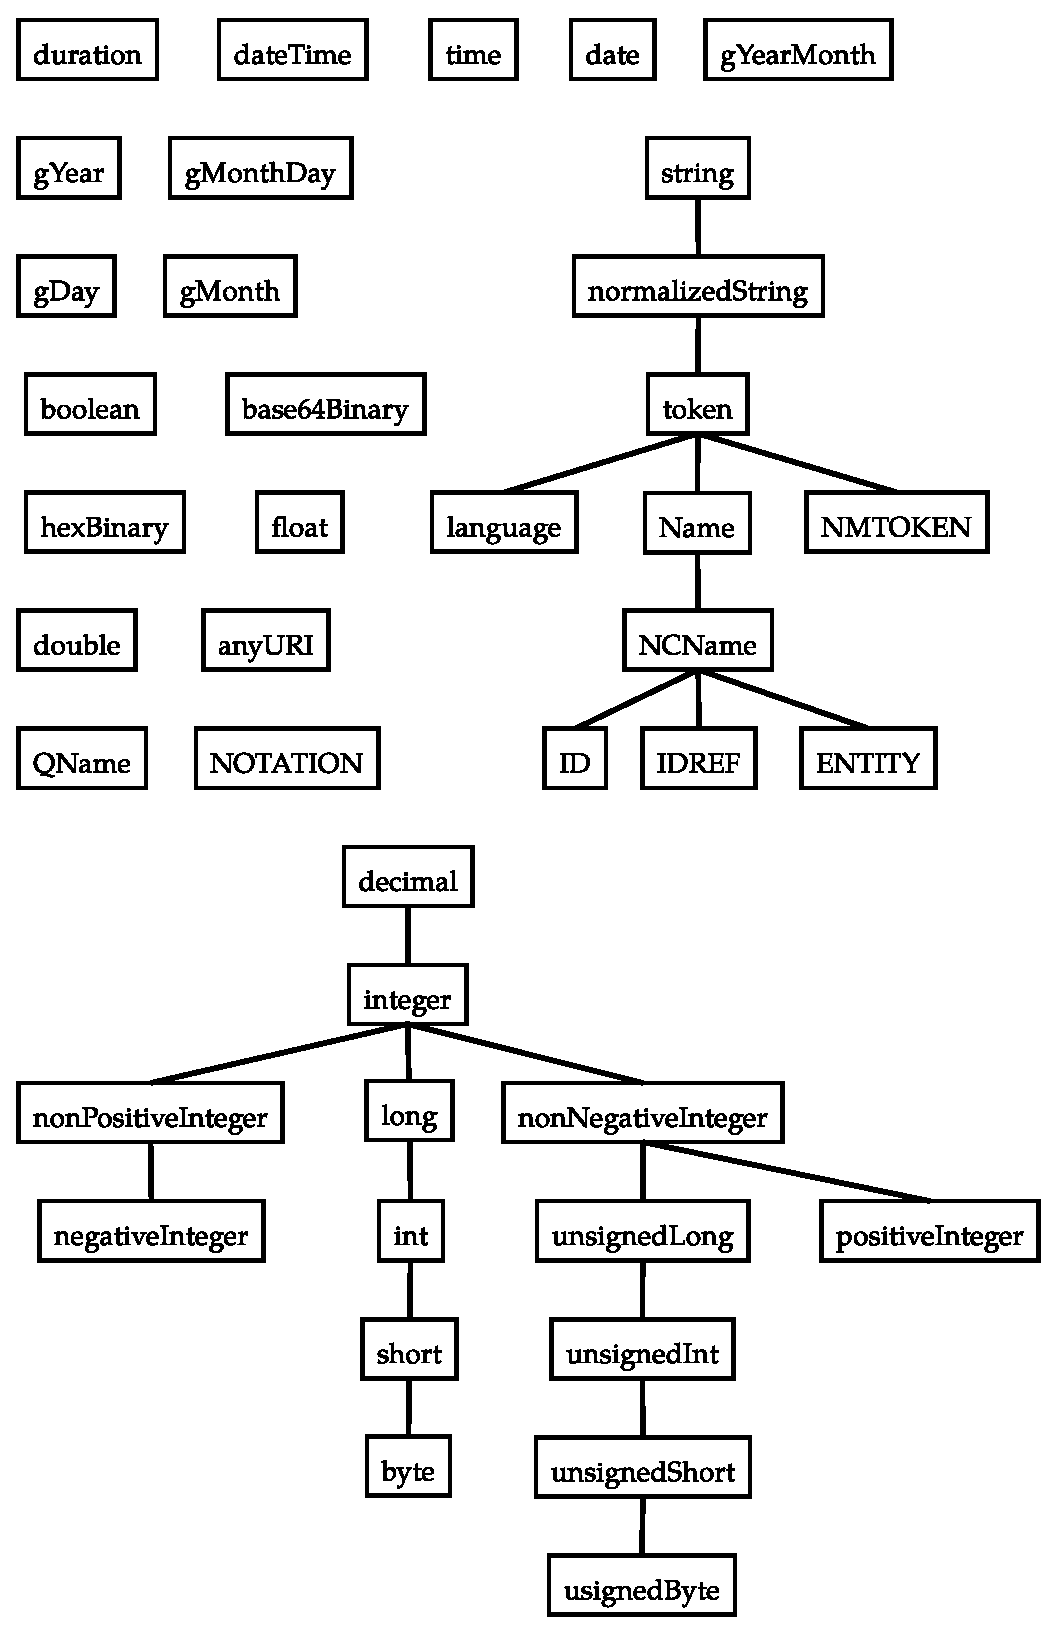
\includegraphics[scale=0.65]{xsd-types.eps}
\end{figure}
